\documentclass[conference]{IEEEtran}
\IEEEoverridecommandlockouts
\usepackage{cite}
\usepackage{amsmath,amssymb,amsfonts}
\usepackage{graphicx}
\usepackage{booktabs}
\usepackage{multirow}
\usepackage{xcolor}
\usepackage{tikz}
\usetikzlibrary{arrows.meta,positioning,shapes.geometric}
\usepackage{url}
\usepackage{balance}
\def\BibTeX{{\rm B\kern-.05em{\sc i\kern-.025em b}\kern-.08em T\kern-.1667em\lower.7ex\hbox{T}\kern-.125emX}}
\newcommand{\pyes}{p_{\mathrm{m}}}
\newcommand{\conf}{c}
\newcommand{\defer}{\mathrm{defer}}

\begin{document}

\title{Learned Deferral for Sanctions Entity Resolution:\\ Classical Matchers, Large Language Models and Human Review}

% TODO: replace e-mail / add roll number if the course template asks for it
\author{\IEEEauthorblockN{Harsh Chauhan}
\IEEEauthorblockA{\textit{Indian Institute of Technology Dharwad}\\
Dharwad, Karnataka, India\\
harsh2005.hc@gmail.com}}

\maketitle

\begin{abstract}
Entity resolution (ER) on sanctions and watch-list data must decide whether two heterogeneous records refer to the same real-world person, company or vessel. The recently released OpenSanctions Pairs benchmark (755{,}540 analyst-judged pairs) reports that the production matcher reaches 91.3\% F1 while frontier LLMs reach up to 99\%, and names \emph{uncertainty-aware review} as the open problem. We revisit this problem from a pattern-recognition standpoint. First, the benchmark lacked a strong classical baseline: a random forest over 29 hand-crafted pair-similarity features reaches 98.7\% test F1, above zero-shot Qwen2.5-7B (95.8\%) and 14B (96.6\%) at a small fraction of the inference cost, and matches the 7B model with only 100 labelled pairs. Second, we cast the match-or-defer decision as Bayes decision theory with a reject option: the calibrated matcher posterior is used to \emph{defer} the least confident pairs to an expert. Deferring 5\% of pairs to a human reviewer removes 71\% of the remaining errors (98.7\,$\rightarrow$\,99.6\% F1); learned gates do not beat this simple confidence rule. Third, using an LLM as the expert yields at most $+0.25$ F1 from a zero-shot 7B model up to a 32B model with chain-of-thought or thinking, because on the deferred pairs every LLM is wrong 18--20\% of the time against the matcher's own 24\%, and a stable core of $\approx$0.5\% of pairs (same-name records with no dates or identifiers) is wrong for every system and, on inspection, is largely irreducible from the record content. Noisy-reviewer and asymmetric-cost analyses, ablations, cross-type generalisation and leakage checks support the conclusions.
\end{abstract}

\begin{IEEEkeywords}
entity resolution, record linkage, reject option, learning to defer, calibration, random forests, large language models, sanctions screening
\end{IEEEkeywords}

\section{Introduction}
Sanctions screening, know-your-customer checks and investigative journalism all depend on \emph{entity resolution} (ER): given two records from different sources, do they describe the same real-world entity? Watch-list records are short, multilingual, inconsistently structured and often transliterated (``Vitaliy Anatolyevich Markelov'' vs.\ ``Witalij Anatoljewicz Markielow''), and mistakes are costly in both directions: a missed match lets a sanctioned party through, a false match blocks an innocent namesake.

OpenSanctions recently released \emph{OpenSanctions Pairs}~\cite{smith2026opensanctions,opensanctions_pairs_docs}, the first large public benchmark for this setting: 755{,}540 analyst-labelled record pairs over more than one million entities from 293 sources in 45 jurisdictions. Their only non-LLM baseline is the production scorer nomenklatura RegressionV1 (91.3\% F1), a simple regression over a handful of hand-written comparison features which the paper labels rule-based, compared against zero- and few-shot LLMs (GPT-4o 99.0\%, DeepSeek-R1-Distill-Qwen-14B 98.2\%) and concludes that pairwise matching is near a practical ceiling, so that future effort should go into blocking, clustering and \emph{uncertainty-aware review}.

Two things are missing from that picture. (i) No modern supervised matcher is reported (the only classical baseline is a linear scorer over a few rule features), although 755k labelled pairs are exactly what feature-based record linkage~\cite{fellegi1969,christen2012} needs. (ii) ``Uncertainty-aware review'' is stated as an open problem but not studied, although it is a textbook instance of \emph{decision theory with a reject option}~\cite{chow1970,bishop2006}: a cheap classifier should abstain on the inputs where its posterior is close to the decision boundary and hand them to a more expensive expert, an LLM or a human analyst.

This project fills both gaps. We ask: (1)~how good is a supervised classical matcher on this benchmark and how many labels does it need; (2)~given a cheap matcher and an expensive expert, \emph{which} pairs should be deferred and how much does deferral buy at a fixed review budget; (3)~are LLM errors complementary to matcher errors, i.e.\ is an LLM a useful expert, and does this change with model size or prompting?

\textbf{Contributions.} (1)~A 29-feature pairwise representation and a comparison of seven classifiers from the PRML syllabus; a random forest reaches 98.7\% test F1 (AUC 0.997), far above the published production scorer and above zero-shot 7B/14B LLMs, with a learning curve. (2)~A reject-option formulation of the match-or-defer decision with confidence, learned, random and oracle gates for two experts (human, LLM), evaluated as deferral curves. (3)~Evidence that matcher and LLM errors are \emph{not} complementary: a $\approx$0.5\% hard core is wrong for every system, and we characterise it. (4)~Ablations, difficulty strata, cross-type generalisation, an entity-overlap leakage analysis and a documented leakage pitfall in the raw benchmark file.

\section{Related Work}
\textbf{Record linkage.} Fellegi and Sunter~\cite{fellegi1969} already define a three-way decision: link, non-link, and \emph{possible link} for clerical review. Practical systems compute string comparators such as Jaro--Winkler~\cite{winkler1990} over aligned fields and learn a decision rule~\cite{christen2012}; deep matchers~\cite{mudgal2018deepmatcher,li2020ditto} and prompted LLMs~\cite{narayan2022wrangle,peeters2025llm} replace the features with learned text representations. The OpenSanctions paper~\cite{smith2026opensanctions} is the first LLM evaluation at this scale on sanctions data.

\textbf{Reject option and learning to defer.} Chow~\cite{chow1970} showed that with known posteriors the Bayes-optimal rule rejects when the maximum posterior falls below a cost-dependent threshold; \cite{herbei2006,cortes2016rejection} analyse learning with rejection and \cite{geifman2017selective} evaluates \emph{selective classification} via risk--coverage curves. \emph{Learning to defer}~\cite{mozannar2020defer} handles an expert who is itself imperfect, so the optimal gate depends on where the expert beats the classifier rather than on confidence alone; our learned ``gain'' gate is of this kind. LLM cascades such as FrugalGPT~\cite{chen2023frugalgpt} route queries between cheap and expensive models with a learned difficulty predictor; here the cheap stage is a classical model and the expensive stage is not clearly stronger.

\section{Data}
\label{sec:data}
\textbf{Source.} We use the public file \texttt{pairs-20251209.json.gz}~\cite{opensanctions_pairs_docs} (755{,}540 lines, as in~\cite{smith2026opensanctions}). Each line holds two FollowTheMoney entities (schema, multi-valued properties such as \texttt{name}, \texttt{alias}, \texttt{birthDate}, \texttt{nationality}, \texttt{idNumber}, \texttt{address}) and an analyst judgement. We keep only entity-level properties and drop provenance fields (\texttt{datasets}, \texttt{referents}, \texttt{first\_seen}, \texttt{target}) that could leak the label.

\textbf{A leakage pitfall.} 280{,}487 lines (37\%) are not analyst judgements of entities but auto-generated \emph{relational stubs} (schemas \texttt{Occupancy}, \texttt{Ownership}, \ldots) whose two sides are byte-identical and always labelled positive. Our first run included them and reported a meaningless 99.4\% F1; inspecting LLM mistakes (``\texttt{Occupancy} vs.\ \texttt{Occupancy}'') revealed the problem. We restrict to the ten entity schemas (Person, Organization, Company, LegalEntity, PublicBody, Vessel, Airplane, Asset, Security, CryptoWallet): 264{,}462 positive and 171{,}380 negative unique unordered pairs (60.7\% positive). Any supervised use of the raw file must apply the same filter.

\textbf{Sample and split.} For tractable LLM inference we draw a uniform random sample of 39{,}000 positive and 21{,}000 negative pairs (60k, 65\% positive) with a fixed seed, and split it 60/10/30 into train (36k), validation (6k) and test (18k). All reported numbers are on the 18k test pairs unless stated otherwise.

\textbf{Leakage checks.} For 53.2\% of test pairs neither entity occurs in training, for 27.1\% one does and for 19.7\% both do (the last group is 99\% negative). The matcher's error rate on fully unseen entities (1.67\%) equals its overall error (1.69\%), so there is no entity memorisation. Only 40 test pairs (0.22\%) duplicate a training pair, and removing the 160 byte-identical test pairs leaves F1 unchanged (98.73 vs.\ 98.72).

\section{Method}
\begin{figure}[t]
\centering
\resizebox{\columnwidth}{!}{%
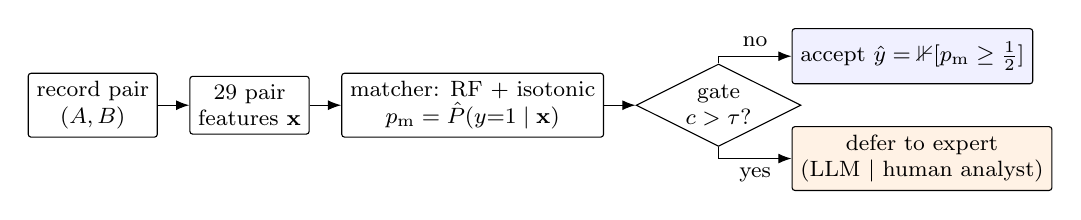
\begin{tikzpicture}[font=\footnotesize,>=Latex,node distance=4mm,
 box/.style={draw,rounded corners=1pt,align=center,inner sep=3pt,minimum height=7mm},
 dec/.style={draw,diamond,aspect=2.0,align=center,inner sep=1pt}]
\node[box] (rec) {record pair\\$(A,B)$};
\node[box,right=of rec] (feat) {29 pair\\features $\mathbf{x}$};
\node[box,right=of feat] (rf) {matcher: RF + isotonic\\$\pyes=\hat P(y{=}1\mid\mathbf{x})$};
\node[dec,right=of rf] (gate) {gate\\$\conf>\tau$?};
\node[box,above right=0mm and 4mm of gate,fill=blue!6] (acc) {accept $\hat y=\mathbb{1}[\pyes\ge\tfrac12]$};
\node[box,below right=0mm and 4mm of gate,fill=orange!10] (exp) {defer to expert\\(LLM $\mid$ human analyst)};
\draw[->] (rec)--(feat); \draw[->] (feat)--(rf); \draw[->] (rf)--(gate);
\draw[->] (gate)|- node[pos=0.75,above]{no} (acc);
\draw[->] (gate)|- node[pos=0.75,below]{yes} (exp);
\end{tikzpicture}}
\caption{The match-or-defer system. The gate score $\conf$ is the matcher's confidence $\min(\pyes,1-\pyes)$ or a learned predictor of matcher error or expert gain; $\tau$ is set by the review budget.}
\label{fig:pipeline}
\end{figure}

\subsection{Pairwise features}
Records are normalised (Unicode transliteration to ASCII, lower-casing, punctuation removal) and all name-like fields (\texttt{name}, \texttt{alias}, \texttt{weakAlias}, \texttt{previousName}) are pooled. We compute 34 features in six groups and use 29 (Table~\ref{tab:feats}): name similarities (maximum over name pairs of Jaro--Winkler, token-set ratio, token Jaccard, Levenshtein ratio; exact normalised-name match; first/last-name overlap), a cross-script flag, entity-type flags, date agreement, geography/gender agreement and conflict, identifier agreement and conflict over 16 identifier fields, address Jaccard and topic/position/birthplace overlap. Five \emph{count} features (numbers of names and properties per side) are excluded from the main model for the reason given in Sec.~\ref{sec:ablation}.

\begin{table}[t]
\caption{Feature groups (29 features used by the matcher).}
\label{tab:feats}
\centering\scriptsize
\begin{tabular}{@{}llp{4.3cm}@{}}
\toprule
Group & \# & Features \\
\midrule
Names & 6 & JW$_{\max}$, token-set$_{\max}$, token-Jaccard$_{\max}$, ratio$_{\max}$, exact normalised name, first/last overlap\\
Script/type & 4 & cross-script, person--person, org--org, type mismatch\\
Dates & 5 & both present, full-date match, year match, min.\ year gap, missing on a side\\
Geography & 6 & both, Jaccard, any overlap, conflict; gender both/mismatch\\
Identifiers & 3 & both present, match, conflict (16 id fields)\\
Other & 5 & address both/Jaccard, topics, position, birthplace overlap\\
\textit{excluded} & 5 & $\log(1{+}\#\text{names}_{L,R})$, $\log(1{+}\#\text{props}_{L,R,\min})$\\
\bottomrule
\end{tabular}
\end{table}

\subsection{Matchers}
We compare seven classifiers~\cite{pedregosa2011sklearn}: logistic regression (standardised, $L_2$), RBF-kernel SVM, $k$-NN ($k{=}25$, distance-weighted), a depth-limited decision tree, random forest (400 trees, min.\ leaf 2, balanced subsampling)~\cite{breiman2001rf}, AdaBoost and histogram gradient boosting, all with balanced class weights. Model selection uses 5-fold stratified cross-validation on the training split, the threshold is tuned on the validation split, and the test split is touched once.

\textbf{Calibration.} Deferral needs probabilities that mean what they say. We fit isotonic regression~\cite{niculescu2005calibration} on the validation split to map the random-forest vote fraction to a calibrated posterior $\pyes$; this lowers the test Brier score from 0.0140 to 0.0137 without changing F1 (98.71\,$\rightarrow$\,98.72).

\subsection{Match or defer as a reject option}
Let $y\in\{0,1\}$ be the true label and $\pyes=\hat P(y{=}1\mid\mathbf{x})$ the calibrated matcher posterior. With a loss of 1 for a wrong decision and a cost $\lambda\in(0,\tfrac12)$ for consulting a perfect expert, the Bayes-optimal rule~\cite{chow1970,bishop2006} is to defer exactly when
\begin{equation}
\conf(\mathbf{x}) = \min(\pyes,\,1-\pyes) \;>\; \lambda ,
\label{eq:chow}
\end{equation}
i.e.\ when the posterior is within $\lambda$ of the decision boundary; the expected risk is $\mathbb{E}[\min(\pyes,1-\pyes)\,\mathbb{1}\{\text{accept}\}]+\lambda\,P(\defer)$. With unequal costs $c_{\mathrm{FP}}$ for a false match, $c_{\mathrm{FN}}$ for a missed match and $c_d$ for review, the three expected losses are $(1-\pyes)c_{\mathrm{FP}}$, $\pyes\,c_{\mathrm{FN}}$ and $c_d$, and the reject region becomes
\begin{equation}
c_d/c_{\mathrm{FN}} \;<\; \pyes \;<\; 1-c_d/c_{\mathrm{FP}} ,
\label{eq:region}
\end{equation}
which shifts towards the cheaper mistake. In practice the analyst capacity is fixed, so we use the equivalent \emph{budget} form: rank test pairs by $\conf$ and defer the top fraction $b$. Reporting system quality as a function of $b$ gives a \emph{deferral curve}, the ER analogue of a risk--coverage curve~\cite{geifman2017selective}.

When the expert is imperfect (an LLM), Eq.~\eqref{eq:chow} is no longer optimal: one should defer where the expert is \emph{more likely to be right than the matcher}~\cite{mozannar2020defer}. We therefore also train two \emph{learned gates} on a 12k slice of the training split for which LLM predictions were collected (disjoint from the matcher's calibration data): an \emph{error gate} $\hat P(\text{matcher wrong}\mid\mathbf{x},\pyes)$ and a \emph{gain gate} $\hat P(\text{LLM right}\wedge\text{matcher wrong}\mid\mathbf{x},\pyes)$, each as logistic regression and as gradient boosting. As bounds we add a \emph{random} gate and an \emph{oracle} gate that defers exactly the pairs the expert would fix.

\subsection{Experts}
\textbf{Human analyst.} Modelled as always correct (the labels \emph{are} analyst judgements), with the review budget $b$ as its cost, which is the production setting of OpenSanctions.

\textbf{LLM.} Qwen2.5-7B-Instruct, Qwen2.5-14B-Instruct and Qwen3-32B (both 4-bit AWQ)~\cite{qwen2025} served with vLLM. Both records are rendered as labelled text blocks inside an analyst-style prompt that asks for a one-word \texttt{yes}/\texttt{no} answer at temperature 0. A 4-shot variant adds two positive and two negative solved examples from a training slice disjoint from all evaluation pairs. Prompts average 417 tokens (1{,}973 with shots); scoring 30k pairs takes 376\,s (7B), 850\,s (14B) and 1{,}934\,s (32B) on an H100 MIG slice, versus 7.7\,s to \emph{train} the forest on a CPU. The 32B model is additionally run with a short chain of thought (``think step by step in at most five sentences, then answer''; 140 output tokens per pair) on the 10\% least confident test pairs, and in its native thinking mode (650 tokens per pair, sampling at temperature 0.6 as recommended) on the 5\% least confident pairs, so that reasoning is spent only where it can matter.

\section{Experiments}
\subsection{Matcher quality}
Table~\ref{tab:matchers} compares classifiers, threshold rules and LLMs on the 18k test pairs. Every learned matcher beats the strongest single-threshold rule (token-set ratio $\ge 0.99$, 94.6\%) and the published production scorer (91.3\%). The random forest is best (98.7\% F1, AUC 0.997) and also better calibrated (Brier 0.014); gradient boosting, $k$-NN and the RBF-SVM are within 0.2 F1, logistic regression trails by 1.6 because several interactions (e.g.\ ``same name \emph{and} conflicting identifier'') are not linearly separable. Zero-shot LLMs are far above the rules but 1.5--3 F1 \emph{below} every non-linear classical matcher. Their published numbers (98--99\% for GPT-4o and a 14B reasoning model) were obtained on a different sample with chain-of-thought decoding, so they are indicative only; our 14B-AWQ with a single-token answer reaches 96.6\%.

\textbf{Not a lucky sample.} Applying the forest trained on the 36k training split to \emph{all} 375{,}842 remaining analyst-judged pairs (60.0\% positive) gives 98.47\% F1 (bootstrap 95\% CI 98.43--98.50), AUC 0.9974 (identical to the test split), precision 97.9 and recall 99.0; the 0.25-point difference to the test split is the lower positive rate acting on precision, not a change in ranking quality. On the same population the best single-threshold rule reaches 94.3\% and logistic regression 96.2\%, and human deferral of 5\% of pairs lifts F1 to 99.56\%.

\begin{table}[t]
\caption{Test results on 18{,}000 pairs (65\% positive). CV = 5-fold out-of-fold F1 on the training split. Matchers use the validation-tuned threshold.}
\label{tab:matchers}
\centering\scriptsize\setlength{\tabcolsep}{3.2pt}
\begin{tabular}{@{}lcccccr@{}}
\toprule
Method & CV F1 & F1 & P & R & AUC & fit\,(s)\\
\midrule
Best rule: token-set ratio $\ge0.99$ & -- & 94.65 & 95.1 & 94.2 & -- & --\\
Published RegressionV1 scorer~\cite{smith2026opensanctions} & -- & 91.3 & -- & -- & -- & --\\
\midrule
Logistic regression & 96.48 & 97.14 & 96.3 & 98.0 & 0.989 & 1.9\\
Decision tree & 98.08 & 98.12 & 97.6 & 98.7 & 0.993 & 0.7\\
AdaBoost & 97.96 & 97.96 & 97.9 & 98.0 & 0.995 & 38.5\\
SVM (RBF) & 98.53 & 98.46 & 98.3 & 98.6 & 0.995 & 13.5\\
$k$-NN ($k{=}25$) & 98.54 & 98.60 & 98.3 & 98.9 & 0.995 & 1.5\\
Gradient boosting & 98.65 & 98.57 & 98.1 & 99.0 & 0.997 & 5.4\\
\textbf{Random forest} (+isotonic) & \textbf{98.69} & \textbf{98.72} & 98.4 & 99.1 & \textbf{0.997} & 7.7\\
\midrule
Qwen2.5-7B, zero-shot & -- & 95.83 & -- & -- & -- & --\\
Qwen2.5-7B, 4-shot & -- & 94.45 & -- & -- & -- & --\\
Qwen2.5-14B-AWQ, zero-shot & -- & 96.58 & -- & -- & -- & --\\
Qwen3-32B-AWQ, zero-shot & -- & 96.77 & -- & -- & -- & --\\
\bottomrule
\end{tabular}
\end{table}

\textbf{Label efficiency.} Fig.~\ref{fig:lc} shows F1 against the number of labelled training pairs. With 100 random labelled pairs the random forest (96.4\%) already exceeds the zero-shot 7B model, with 200 it exceeds the 14B model, and it keeps improving to 36k pairs; logistic regression saturates near 96.5\%. Hand-crafted similarity features are an extremely strong prior for this task.

\begin{figure}[t]
\centering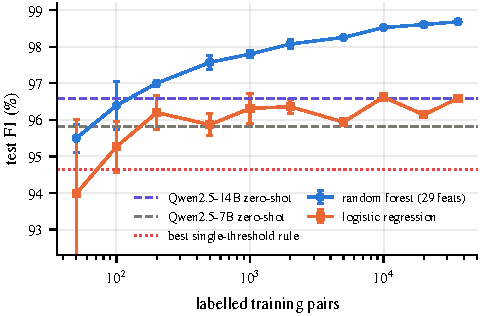
\includegraphics[width=0.9\columnwidth]{fig_learning_curve.pdf}
\caption{Learning curve (test F1 vs.\ labelled pairs, log scale; error bars over 3 draws for $n<5000$).}
\label{fig:lc}
\end{figure}

\subsection{Feature ablation and a dataset artefact}
\label{sec:ablation}
Table~\ref{tab:ablation} removes feature groups. Names alone give 97.0\%; adding attribute agreement/conflict features brings the remaining 1.7 points, and attributes without any name feature still reach 97.4\%, so the two sources are complementary. The five \emph{count} features alone reach 85.7\% F1, far above chance, although they say nothing about whether two records agree. Class-conditional statistics explain why: negatives are drawn around large merged clusters, so the negative side has on average $e^{1.63}{-}1\approx4$ names versus $\approx1.7$ for positives. This is a benchmark artefact rather than evidence, so the main model excludes these features (costing 0.3 F1). It mirrors the relational-stub issue of Sec.~\ref{sec:data}: a learned matcher will exploit any construction bias of a pairs file.

\begin{table}[t]
\caption{Feature-group ablation (RF test F1, \%; LR in parentheses).}
\label{tab:ablation}
\centering\scriptsize
\begin{tabular}{@{}lcc@{}}
\toprule
Feature set & \# & F1 \\
\midrule
all 34 (incl.\ counts) & 34 & 98.99 (97.16)\\
\textbf{no counts (main model)} & 29 & 98.69 (96.59)\\
no counts, no topics & 28 & 98.55 (96.52)\\
names only & 6 & 96.98 (94.33)\\
names + dates & 11 & 97.30 (94.97)\\
attributes only (no names) & 28 & 97.42 (93.89)\\
counts only & 5 & 85.68 (77.78)\\
all but exact-name flag & 33 & 99.00 (97.13)\\
\bottomrule
\end{tabular}
\end{table}

\subsection{Are LLM and matcher errors complementary?}
Table~\ref{tab:comp} decomposes the test pairs by who is right. With the 7B model, the matcher alone is right on 4.67\% of pairs, the LLM alone on 1.03\%, and both are wrong on 0.66\%. A system that could pick the right oracle per pair would therefore reach $\approx$99.5\% F1 (118 remaining errors), but only by identifying the 1.03\% LLM-only pairs, which is the ceiling of LLM deferral. Doubling the LLM (14B) or adding 4-shot examples moves the first number but leaves the LLM-only and both-wrong shares essentially fixed (1.05\%/0.64\% and 1.03\%/0.66\%): larger or better-prompted models fix pairs the matcher already got right. The 32B model is the best LLM alone (96.8\%) yet has the \emph{smallest} LLM-only share (0.88\%) and the largest both-wrong share (0.81\%). Few-shot prompting actually hurt the 7B model (95.8\,$\rightarrow$\,94.5\% F1), a known failure mode of small instruction-tuned models.

\begin{table}[t]
\caption{Error decomposition on the 18k test pairs (\%), matcher fixed.}
\label{tab:comp}
\centering\scriptsize\setlength{\tabcolsep}{3.5pt}
\begin{tabular}{@{}lcccc@{}}
\toprule
LLM configuration & both right & matcher only & LLM only & both wrong\\
\midrule
Qwen2.5-7B, zero-shot & 93.64 & 4.67 & 1.03 & 0.66\\
Qwen2.5-14B, zero-shot & 94.55 & 3.76 & 1.05 & 0.64\\
Qwen2.5-7B, 4-shot & 91.99 & 6.32 & 1.03 & 0.66\\
Qwen3-32B, zero-shot & 94.93 & 3.38 & 0.88 & 0.81\\
\bottomrule
\end{tabular}
\end{table}

\subsection{Deferral curves}
Fig.~\ref{fig:defer} and Table~\ref{tab:defer} give the main result. \textbf{Human expert (a).} The confidence gate of Eq.~\eqref{eq:chow} is remarkably effective: deferring 1\% of pairs removes 22\% of the matcher's 304 errors, 2\% removes 34\%, 5\% removes 71\% (99.63\% F1) and 10\% removes 85\% (99.81\%). The oracle needs 1.7\% to remove all errors; a random gate at 5\% removes 5\%. The learned error gate matches the plain confidence rule at 1--2\% and is slightly \emph{worse} from 5\% on (99.51 vs.\ 99.63), and the confidence score has the highest AUC for predicting matcher error (0.945 vs.\ 0.932 for gradient boosting): the calibrated posterior already carries the available information about its own mistakes, as Chow's rule assumes.

\textbf{LLM expert (b).} Deferring to the 7B model helps only at small budgets and peaks at $+0.14$ F1 (5\%); beyond $\approx$8\% the system is worse than not deferring, and at 100\% it degrades to the LLM's own 95.8\%. Even the oracle gate gains only $+0.76$ at 1\% and declines afterwards, because there are few LLM-only pairs to find. Learned gain gates reach $+0.23$ at 3\%, the 14B model $+0.23$ at 5\%; the 4-shot model gives nothing beyond 1\% with the confidence gate. Comparing the panels at an equal 5\% budget: a human removes 217 errors, the best LLM removes 54.

\begin{figure*}[t]
\centering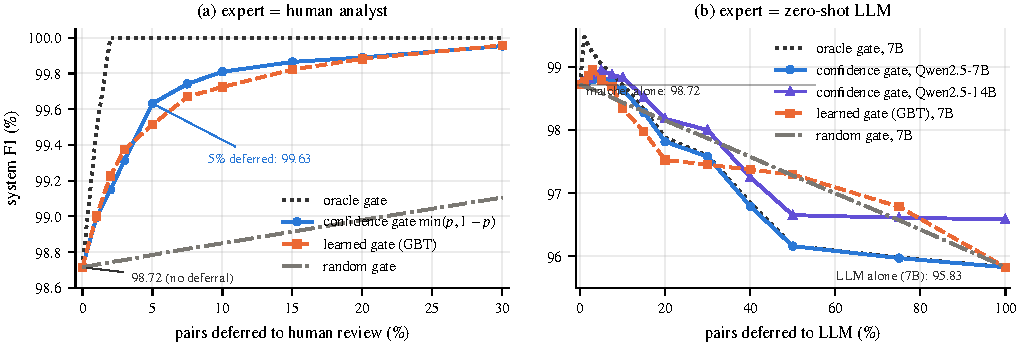
\includegraphics[width=0.86\textwidth]{fig_deferral.pdf}
\caption{Deferral curves on the 18k test pairs. (a) Human expert: system F1 as the least confident pairs are sent to review; (b) LLM expert: the same with a zero-shot LLM answering the deferred pairs. Note the different axis ranges.}
\label{fig:defer}
\end{figure*}

\begin{table}[t]
\caption{System F1 (\%) at fixed deferral budgets (test). Base matcher: 98.72.}
\label{tab:defer}
\centering\scriptsize\setlength{\tabcolsep}{3.5pt}
\begin{tabular}{@{}llcccc@{}}
\toprule
Expert & Gate & 1\% & 2\% & 5\% & 10\%\\
\midrule
\multirow{4}{*}{human} & random & 98.73 & 98.74 & 98.78 & 98.85\\
 & confidence $\min(p,1{-}p)$ & \textbf{98.99} & 99.15 & \textbf{99.63} & \textbf{99.81}\\
 & learned error gate (GBT) & 99.00 & \textbf{99.23} & 99.51 & 99.73\\
 & oracle & 99.47 & 100 & 100 & 100\\
\midrule
\multirow{4}{*}{LLM 7B} & confidence & 98.76 & 98.78 & 98.85 & 98.63\\
 & learned gain gate (GBT) & 98.76 & 98.86 & 98.79 & 98.34\\
 & oracle & 99.48 & 99.33 & 99.05 & 98.72\\
\multirow{1}{*}{LLM 14B} & confidence & 98.77 & 98.82 & 98.94 & 98.83\\
\multirow{1}{*}{LLM 7B 4-shot} & confidence & 98.77 & 98.72 & 98.69 & 98.30\\
\bottomrule
\end{tabular}
\end{table}

\subsection{Scaling the expert}
Table~\ref{tab:experts} asks whether a larger model with explicit reasoning changes the picture at the budget where LLM deferral peaks (5\%). It does not: zero-shot Qwen3-32B gives $+0.14$, chain of thought $+0.22$ and thinking mode $+0.25$ F1, against $+0.91$ for the human. The explanation is one column of the table. On the deferred pairs every LLM, from 7B zero-shot to 32B thinking, is wrong 18--20\% of the time, while the matcher itself is wrong 24\% of the time there, and deferral pays only in proportion to how far the expert beats the matcher on the pairs it receives. The thinking model fixes 141 of the 217 matcher errors in the deferred set but introduces 82 new ones, and recovers 9 of the 89 hard-core pairs of Sec.~\ref{sec:core}; its 650 reasoning tokens per pair buy 0.1 F1 over 14B zero-shot.

\begin{table}[t]
\caption{Experts on the 5\% least confident test pairs (900 pairs, 217 matcher errors). Alone: expert F1 on the full test set. At 5\%: system F1 with the expert answering the deferred pairs. Fixed/broken: matcher errors corrected / correct decisions overturned. Err.: expert error rate (\%) on the deferred pairs (matcher: 24.1). Core: hard-core pairs (of 89) the expert gets right.}
\label{tab:experts}
\centering\scriptsize\setlength{\tabcolsep}{2.2pt}
\begin{tabular}{@{}lcccccc@{}}
\toprule
Expert & alone & at 5\% & errors & fixed/broken & err.\ & core\\
\midrule
Qwen2.5-7B 0-shot & 95.83 & 98.85 & 271 & 145/112 & 20.4 & 0\\
Qwen2.5-14B 0-shot & 96.58 & 98.94 & 250 & 147/93 & 18.1 & 0\\
Qwen2.5-7B 4-shot & 94.45 & 98.69 & 308 & 146/150 & 24.6 & 0\\
Qwen3-32B 0-shot & 96.77 & 98.86 & 270 & 118/84 & 20.3 & 4\\
Qwen3-32B chain of thought & -- & 98.93 & 253 & 143/92 & 18.4 & 4\\
Qwen3-32B thinking & -- & 98.97 & 245 & 141/82 & 17.6 & 9\\
\midrule
Human analyst & -- & \textbf{99.63} & 87 & 217/0 & 0 & --\\
\bottomrule
\end{tabular}
\end{table}

\subsection{Imperfect reviewers, asymmetric costs, combination}
\textbf{Noisy reviewer.} Flipping each reviewed label with probability $\epsilon$ (20 draws) gives, at the 5\% budget, 99.55\% F1 for $\epsilon=2\%$, 99.45 for 5\%, 99.25 for 10\% and 98.87 for 20\%, all above the 98.72 baseline: any reviewer who beats the matcher's 24\% error on the deferred pairs helps, which places the LLMs of Table~\ref{tab:experts} at the margin.

\textbf{Asymmetric costs.} Eq.~\eqref{eq:region} with $c_{\mathrm{FP}}=1$, $c_{\mathrm{FN}}=10$ and $c_d=0.1$ gives the reject region $0.01<\pyes<0.9$: 10.7\% of pairs are deferred, missed matches fall from 24 to 3, and the realised cost per 1000 pairs falls from 37.9 (best single threshold without a reject option, at $\pyes\ge0.09$) to 15.6. With equal costs and $c_d=0.1$ the region is $[0.1,0.9]$, 5.3\% are deferred and the cost falls from 16.8 to 9.9.

\textbf{Combining instead of deferring.} Using the 7B LLM's $P(\text{yes})$ together with the matcher lands in the same place: a weighted average tuned on the 12k gate-training pairs gives 98.89, a logistic stacker on both logits 98.90, and a forest with $P(\text{yes})$ as a 30th feature 98.86 (98.52 without it on the same 12k pairs). The LLM carries about 0.2 F1 of information, however it is used.

\subsection{Who gets deferred, and the hard core}\label{sec:core}
The 10\% of test pairs deferred by the confidence gate differ systematically from the rest: 84\% lack a date on at least one side (vs.\ 40\%), 55\% are organisation pairs (vs.\ 33\%), 12\% are cross-script (vs.\ 7\%), and both systems fail on them often (matcher error 14.4\% vs.\ 0.3\%, LLM error 15.4\% vs.\ 4.2\%). To see what no system can do, we intersect the error sets: of the 304 matcher errors, 115--119 are also errors of each LLM configuration, and 89 pairs (0.49\% of the test set) are wrong for all four systems. Fig.~\ref{fig:core} (left) profiles this core: 85\% have no date on a side, only 18\% have identifiers on both sides, and 63\% share an exact normalised name, yet 79\% were judged \emph{negative} by analysts while the matcher says match on 79\% of them. Inspection shows namesakes with no distinguishing attribute (e.g.\ two byte-identical Thai legislator records labelled not-same), which require knowledge outside the records, and a few apparent label errors (identical birth date and birthplace labelled not-same). 42\% of the core is misclassified with confidence $\max(\pyes,1-\pyes)\ge0.95$ and is therefore unreachable by any confidence-based gate; the remainder is caught early (56\% of the core lies in the 5\% least confident pairs, 72\% in the 10\%). This supports treating $\approx$0.5\% as the information floor of the benchmark and sending exactly such pairs to review as the principled policy.



\subsection{Difficulty strata and generalisation}
\textbf{Strata.} 56\% of test pairs share an exact normalised name (97.5\% positive) and 44\% do not (23.9\% positive). The matcher scores 99.2\% and 96.1\% on the two halves, while the LLMs fall to 88--89\% on the hard half and to 84--85\% when additionally JW$_{\max}<0.9$: transliterated and differently spelled names are where learned string comparators beat the LLM most. Human deferral is equally effective on the hard half alone (96.1\,$\rightarrow$\,98.6\% at 5\%, 99.5\% at 10\%).

\begin{figure}[t]
\centering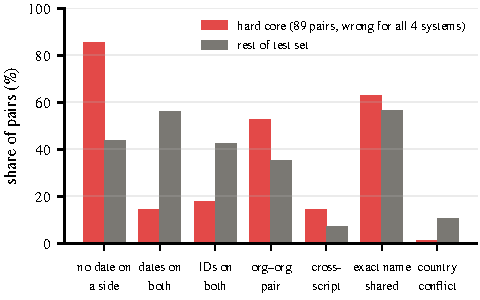
\includegraphics[width=0.88\columnwidth]{fig_core.pdf}
\caption{Attribute profile of the 89 hard-core test pairs against the rest of the test set.}
\label{fig:core}
\end{figure}

\textbf{Per type.} Matcher vs.\ 7B error rates are 1.1\% vs.\ 3.1\% on person pairs, 2.9\% vs.\ 9.0\% on organisation pairs, 2.9\% vs.\ 15.2\% on cross-script pairs, 0.5\% vs.\ 3.3\% when both sides carry a date and 3.2\% vs.\ 7.8\% when one does not; the ordering agrees with the published observation that LLMs struggle with transliteration~\cite{smith2026opensanctions}.

\textbf{Cross-type generalisation.} A forest trained only on 22k person pairs transfers to the 6.4k organisation test pairs at 90.0\% (vs.\ 97.1\% for the full model), organisation-trained models transfer to persons at 97.8\% (99.3\%), and training on same-script pairs only still gives 97.1\% on the 1.3k cross-script pairs (98.3\%). The features are largely type-agnostic, but person-specific cues (dates, gender) do not substitute for organisation cues (registration numbers, jurisdictions).


\section{Discussion and Limitations}
\textbf{What the results mean.} The ``LLM vs.\ rules'' framing hides a stronger and far cheaper alternative: a non-linear supervised matcher on similarity features (our own logistic regression on the same features reaches 97.1\%, so the gap to the published 91.3\% is mostly about features and training). The real open problem is deciding \emph{which} pairs a human must see, and the textbook answer, calibrate and then reject near the boundary, is close to the oracle on the first few percent of the budget. An LLM is not a good stand-in for the human, not because it is weak on average but because it is weak on the \emph{same} pairs, and neither model size (7B to 32B) nor reasoning (chain of thought, thinking mode) changes this: on the deferred pairs its error rate stays within a few points of the matcher's own. 

\textbf{Limitations.} (i)~Our LLMs are open models up to 32B; frontier models reach 98--99\%~\cite{smith2026opensanctions} and might err differently, although the hard-core analysis and the flat error rate on deferred pairs from 7B to 32B with reasoning suggest the floor is informational. (ii)~The human expert is assumed perfect; the noisy-reviewer analysis shows the gain survives 10--20\% reviewer error, but several core pairs look like label noise, which caps every system. (iii)~We use a 60k uniform sample whose class ratio (65\% positive) is far from the production ratio after blocking, so absolute F1 values are not deployment estimates, although deferral \emph{rankings} are insensitive to the prior. (iv)~Pairwise decisions ignore the clustering step, and we use one benchmark in one domain.

\section{Conclusion}
We built a match-or-defer system for sanctions entity resolution on the OpenSanctions Pairs benchmark. A random forest over 29 hand-crafted pair features reaches 98.7\% F1, above zero-shot 7B/14B LLMs and the published production scorer, with only hundreds of labels needed. Treating review as a reject option, a calibrated-confidence gate lets a human remove 71\% of the remaining errors by examining 5\% of pairs; learned gates add nothing, a reviewer wrong 10\% of the time still helps, and the same rule adapts to asymmetric costs. LLM deferral yields at most $+0.25$ F1 from 7B zero-shot to 32B with reasoning, whether the LLM is deferred to or combined with the matcher, because its error rate on the deferred pairs stays near the matcher's own and matcher and LLM errors coincide on a $\approx$0.5\% core of attribute-poor same-name pairs that is irreducible from record content. Two construction artefacts of the benchmark file (relational stubs, cluster-size counts) inflate supervised scores if not removed. Future work: frontier models on the deferred pairs, evaluation at the deployment class ratio, type-aware hybrid routing, and extending the reject option to clustering. All code accompanies this report as plain Python scripts with fixed seeds and an executed notebook; the data file is public~\cite{opensanctions_pairs_docs}, and everything except LLM inference runs in minutes on a CPU.

\balance
\bibliographystyle{IEEEtran}
\bibliography{refs}

\end{document}
